\section{Empirical Motivation}
\label{sec:motivation-empirical}

To motivate provider-level routing, we profile three web-search providers---Tavily,
Brave, and DuckDuckGo---on $200$ questions from HotpotQA and TriviaQA. All three
are called through the same \texttt{web\_search} interface, so observed
differences reflect the provider, not the call site.

\begin{figure}[t]
\centering
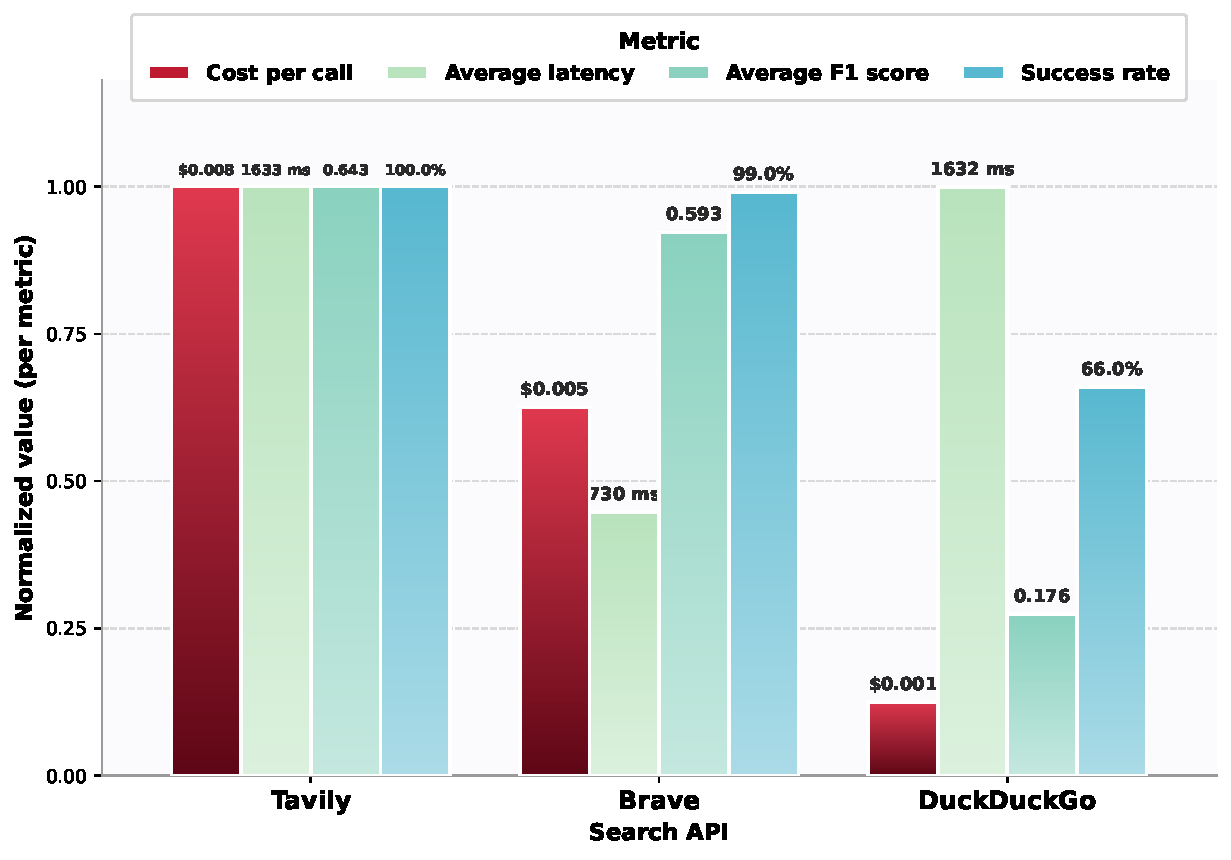
\includegraphics[width=\linewidth]{figs/search_api_metrics.pdf}
\caption{Per-provider cost, latency, F$_1$, and success rate.
Bars are min--max normalised; in-bar labels show raw values.}
\label{fig:api-metrics}
\end{figure}

\paragraph{Providers differ on every axis.} Figure~\ref{fig:api-metrics} shows
that the three providers occupy distinct points in cost, latency, F$_1$, and
success rate. The usual cost--quality correlation holds only in aggregate;
neither cost nor latency alone identifies the best provider for a given query.

\begin{figure}[h]
    \centering
    \begin{subfigure}{0.32\linewidth}
        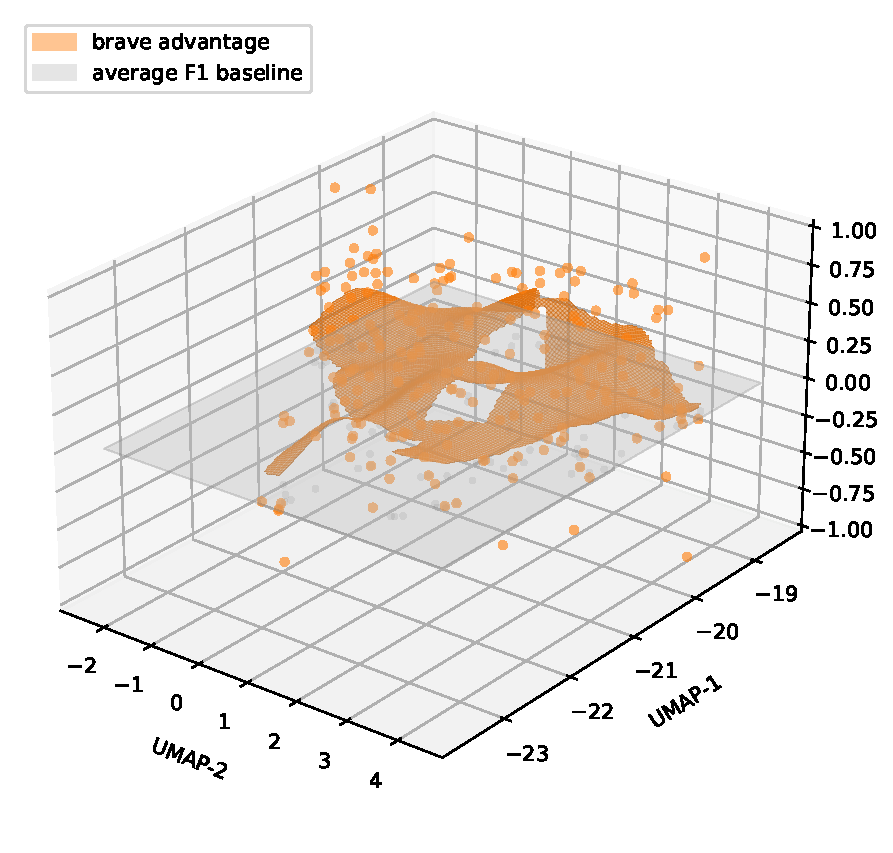
\includegraphics[width=\linewidth]{figs/search_api_umap_brave_advantage.pdf}
        \caption{Brave}
    \end{subfigure}\hfill
    \begin{subfigure}{0.32\linewidth}
        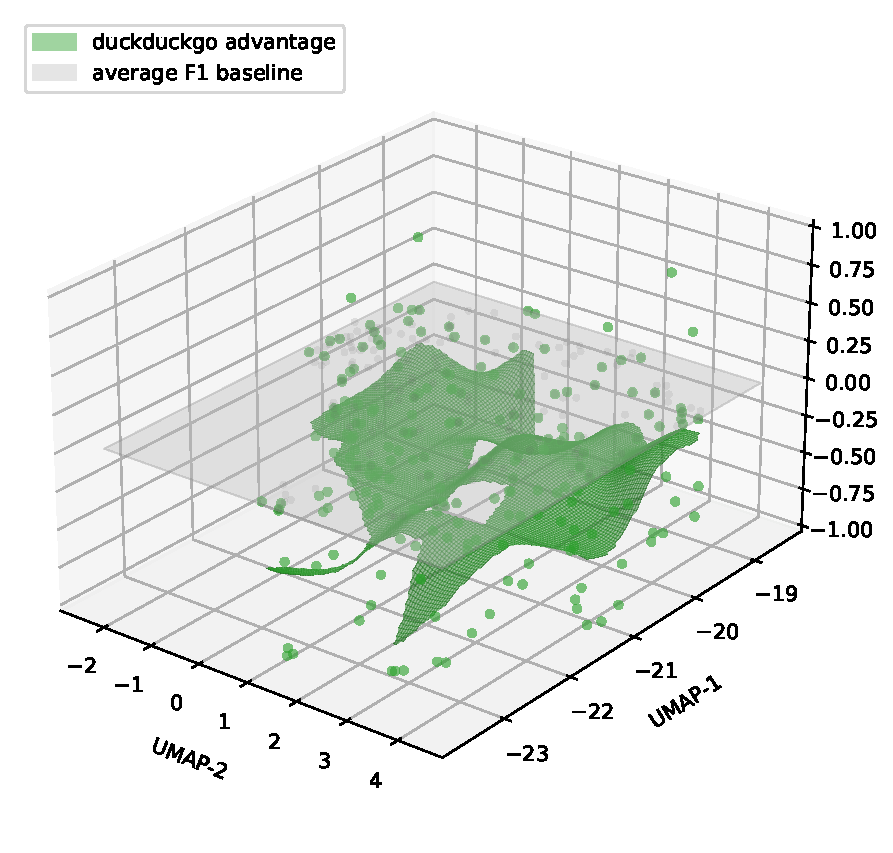
\includegraphics[width=\linewidth]{figs/search_api_umap_duckduckgo_advantage.pdf}
        \caption{DuckDuckGo}
    \end{subfigure}\hfill
    \begin{subfigure}{0.32\linewidth}
        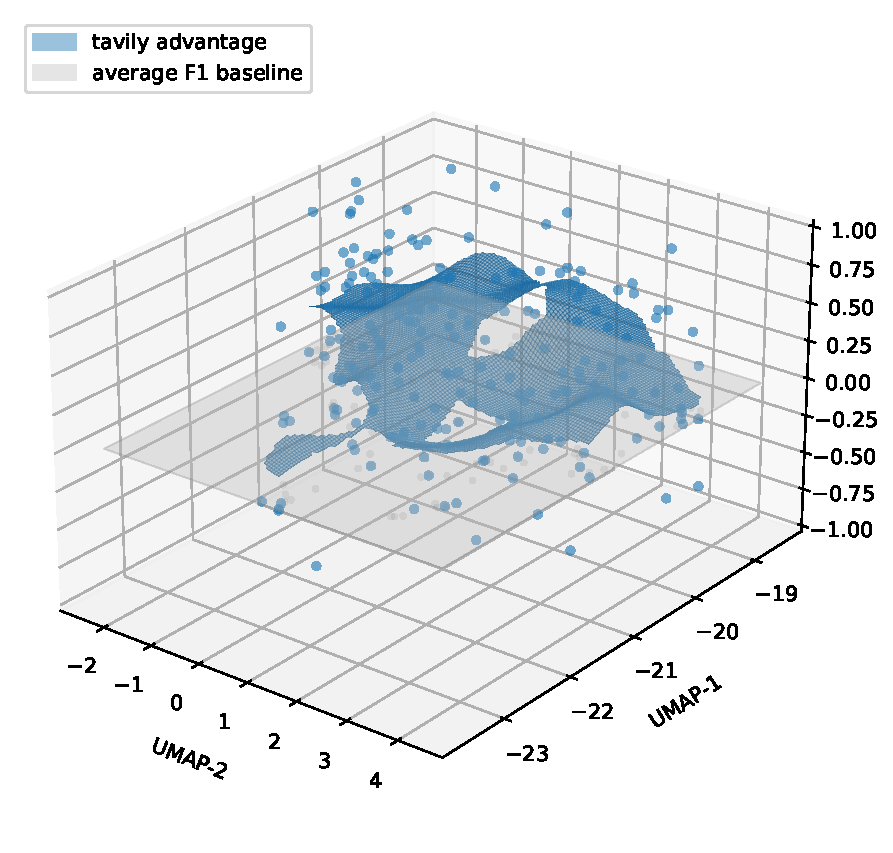
\includegraphics[width=\linewidth]{figs/search_api_umap_tavily_advantage.pdf}
        \caption{Tavily}
    \end{subfigure}
    \caption{Per-provider F$_1$ advantage over the other two, plotted on the
    UMAP embedding of the query.}
    \label{fig:umap_three-subfigures}
\end{figure}

\paragraph{Quality is query-specific.} Embedding queries and projecting them
with UMAP (Figures~\ref{fig:umap_three-subfigures},~\ref{fig:umap}) reveals two
patterns: many queries are ties across all three providers, and the non-tied
winners are scattered rather than clustered. Tavily wins most often overall,
but Brave and DuckDuckGo each dominate on substantial subsets that are not
separable by coarse query type.

\begin{figure}[ht]
\centering
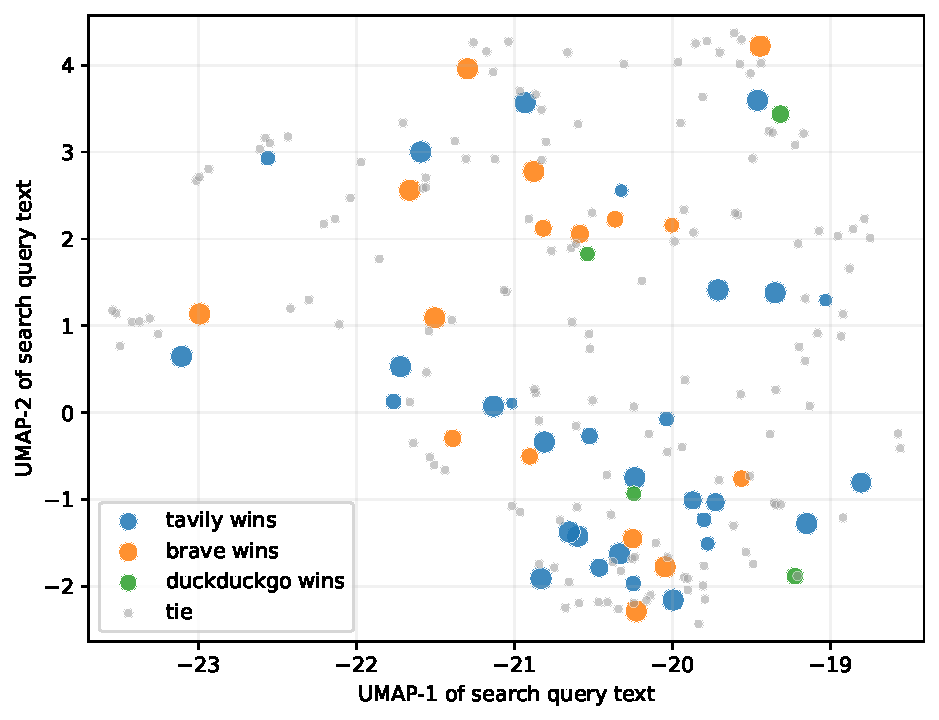
\includegraphics[width=0.78\linewidth]{figs/search_api_umap_best_api_map.pdf}
\caption{UMAP of query embeddings, coloured by the highest-F$_1$ provider.
Grey points are ties.}
\label{fig:umap}
\end{figure}

\paragraph{Routing dominates any fixed-provider policy.}
Figure~\ref{fig:oracle} compares single-provider policies against a per-query
oracle that picks the highest-F$_1$ provider within a $1065$~ms SLO, breaking
ties by cost. Any fixed choice trades cost for quality; the oracle cuts cost
by $37.5\%$ \emph{and} improves F$_1$ by $11.8\%$ over the best single-provider
baseline by spending the expensive provider only where it matters.

\begin{figure}[t]
\centering
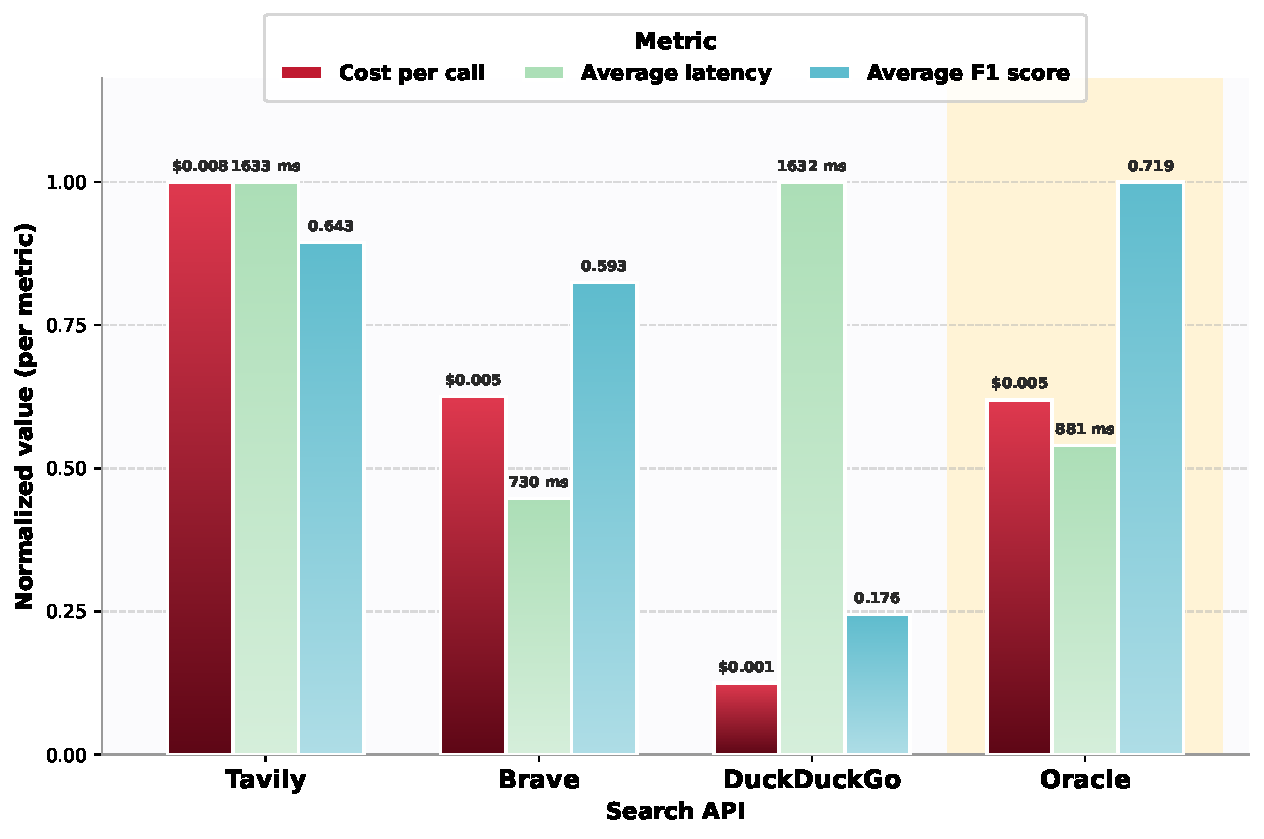
\includegraphics[width=\linewidth]{figs/search_api_oracle_comparison.pdf}
\caption{Single-provider policies vs.\ the per-query oracle (SLO $1065$~ms,
ties broken by cost).}
\label{fig:oracle}
\end{figure}

These observations motivate a per-query router. The remaining question is how
to approximate the oracle online, without gold labels and under non-stationary
load---the problem addressed in the rest of the paper.